


\section{The COVID Recession and Temporary Layoffs}


\subsection{The COVID Recession and the Absence of Scarring}

The behavior of unemployment during the COVID recession was unprecedented due to various reasons. One of these reasons is that 97.7$\%$ of the increase in the unemployment rate was attributed to temporary layoffs \citep{Gertler2022}. In this section, I show that, during the COVID recession, unemployment scarring did not translate to macro scarring because of the unprecedented fraction of temporary layoffs . Further, this section also shows that the model can explain both recessions with sluggish recoveries as well as recessions with quick recoveries. I repeat the estimation procedure of the previous section and recalibrate $\zeta^{X}$ for each unemployment state X to maximize the proportion of temporary layoffs that is attributed to a change in the unemployment rate. Further I assume that temporary layoffs cannot transition to a permanent layoff by setting $P_{TLPL} = 0$.\footnote{\cite{Gertler2022} note that 98$\%$ of these temporary layoffs do not transition to a permanent layoff.} At best, the model can attribute 78.5$\%$ of an increase in the unemployment rate to temporary layoffs.  Figure \ref{COVID_recession} plots the responses of unemployment rate, Gini index for income, consumption, output under the model with scarring calibrated to maximize the proportion of temporary layoffs (purple), and the version of the model without scarring (orange). With a large mass of temporary layoffs, the effects of unemployment scarring are effectively eliminated as temporary layoffs are reemployed at their pre-job layoff wage. The effective absence of unemployment scarring reduces the persistence of the responses of consumption and output in the baseline model leading leading the model to be consistent with the empirical paths of consumption and GDP. Further, the response of the Gini index is transitory, similar to the data. 

 

\begin{figure}[t!] % "[t!]" placement specifier just for this example
\centering
\begin{minipage}{0.51\textwidth}
\includegraphics[scale=.57]{text/chapter1/Figures/pandemic_sim/Urate_pandemic}
 \label{fig:a}
\end{minipage}\hspace*{\fill}
\begin{minipage}{0.51\textwidth}
\includegraphics[scale=.57]{text/chapter1/Figures/pandemic_sim/income_gini_pandemic}
 \label{fig:b}
\end{minipage}




\medskip
\begin{minipage}{0.51\textwidth}
\includegraphics[scale=.57]{text/chapter1/Figures/pandemic_sim/C_pandemic}
\label{fig:c}
\end{minipage}\hspace*{\fill}
\begin{minipage}{0.51\textwidth}
\includegraphics[scale=.57]{text/chapter1/Figures/pandemic_sim/GDP_pandemic}
 \label{fig:d}
\end{minipage}
\caption{Model vs data: The COVID Recession}
\floatfoot{Note: In this exercise, the effects unemployment scarring are eliminate when the model is recalibrated to match the large proportion of temporary layoffs that explain the rise in unemployment. In particular, for this calibration, 78.5 $\%$ of the increase in the unemployment rate is attributed to temporary layoffs. Empirically, $97.7 \%$ of the increase in the unemployment rate is due to temporary layoffs. The model is unable to account for such a large proportion of temporary layoffs because the fall in labor market tightness during the simulation lowers the job finding probability of those who were already in a  permanently layoff prior to the recession. Thus, the duration of those permanent layoffs rises.}

\label{COVID_recession}

\end{figure}



\subsection{Temporary Layoffs and Swift Recoveries}


In this section, I demonstrate that temporary layoffs,  following the COVID recession,  were instrumental in both accelerating the swift recovery of GDP and in preventing a permanent rise in income inequality. To show this, I repeat the estimation procedure of matching the unemployment rate during the COVID Recession but recalibrate the model to maximize the fraction of permanent layoffs that can be attributed to an increase in the unemployment rate. Because the job probabilities of workers who are in temporary layoff falls endogenously with the unemployment rate, the duration of a temporary layoff rises therefore preventing the model from producing an increase in an unemployment rate that is entirely explained by permanent layoff.\footnote{In other words, even if the increase in the EU probability in this simulation is completely captured by permanent layoffs, the UE probability of workers who were in temporary layoff prior to the recession must also fall.}

Figure \ref{COVID_Counterfactual_GDP} and figure \ref{COVID_Counterfactual_gini} compares the path of output and income Gini, respectively, under the original calibration (from section 9.1) against the counterfactual scenario with a large fraction of permanent layoffs. In all lines in each figure, the path of unemployment remains identical and instead only differs in the composition of the unemployment rate between permanent and temporary layoffs. Figure \ref{COVID_Counterfactual_GDP} demonstrates that if the rise in unemployment has been primarily due to permanent layoffs, GDP would not have returned to its pre-recessionary trend. Although the long run difference between the counterfactual and the data may appear small ---due to the sharp initial contraction in GDP--- the percentage deviation of the counterfactual from the trend reaches 2 $\%$ by the second quarter of 2023. This magnitude is within range of long run output deviations observed after the 1990-1991 and 2000s recessions. Moreover, emphasizing the role of temporary layoffs does not diminish the significance of fiscal policy in shaping the recovery from the pandemic. Fiscal measures may have contributed to the large proportion of temporary layoffs during the COVID Recession. Overall, temporary layoffs were a key factor in enabling GDP to return to its pre-recessionary trend and likely complemented the effectiveness of fiscal stimulus during this period. Similarly, Figure \ref{COVID_Counterfactual_gini} illustrates that temporary layoffs prevented the permanent rise in the Gini index for income. Notably, the red line demonstrates that if the majority of the increase in the unemployment rate was due to permanent layoffs, then the Gini index for income would have permanently risen.  




\begin{figure}[!ht!]
\begin{center}
\includegraphics[scale=.53]{text/chapter1/Figures/pandemic_counterfactual/output_vs_data_jam_COVID_counterfactual}
\end{center}
\caption{Counterfactual for GDP: What if the rise in unemployment during the pandemic was due to permanent layoffs? }
\floatfoot{This figure plots the paths of output with trend from the HANK + Scarring model (purple) under the baseline COVID calibration (with 78$\%$ temporary layoffs) against a counterfactual (red) where the rise in unemployment during COVID is largely explained by permanent layoffs. Note that for both paths of output, the unemployment rate is identical. Only the composition of the unemployment rate differs. }
\label{COVID_Counterfactual_GDP}
\end{figure}



\begin{figure}[!ht!]
\begin{center}
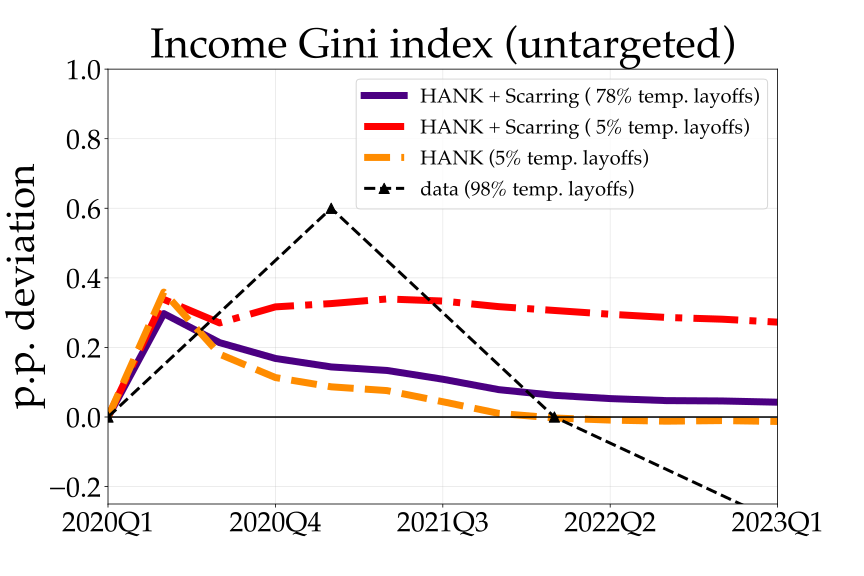
\includegraphics[scale=.53]{text/chapter1/Figures/pandemic_counterfactual/income_gini_pandemic_counterfactual_perm_only}
\end{center}
\caption{Counterfactual for Gini index: What if the rise in unemployment during the pandemic was due to permanent layoffs?}
\floatfoot{This figure plots the paths of the income Gini index from the HANK + Scarring model (purple) under the baseline COVID calibration (with 78$\%$ temporary layoffs) against a counterfactual (red) where the rise in unemployment during COVID is largely explained by permanent layoffs. Note that for both paths of the income Gini index, the unemployment rate is identical. Only the composition of the unemployment rate differs. }
\label{COVID_Counterfactual_gini}
\end{figure}


